\chapter{Introduction}

Nuclear physics aims to understand systems
where the structure and dynamics are dominated by the strong interaction,
one of the four fundamental forces of nature.
The goals of nuclear science are well-described by the overarching open questions
identified by the U.S.~National Academy of Science in \textit{Exploring the Heart of Matter}~\cite{NRC13heartofmatter}:
\begin{enumerate}
  \item How did matter come into being and how does it evolve?
  \item How does subatomic matter organize itself and what phenomena emerge?
  \item Are the fundamental interactions that are basic to the structure of matter fully understood?
  \item How can the knowledge and technological progress provided by nuclear physics best be used to benefit society?
\end{enumerate}
At the heart of this work is the second question,
with the focus of our attention being on the structure of atomic nuclei.

\begin{figure}[t]
  \centering
  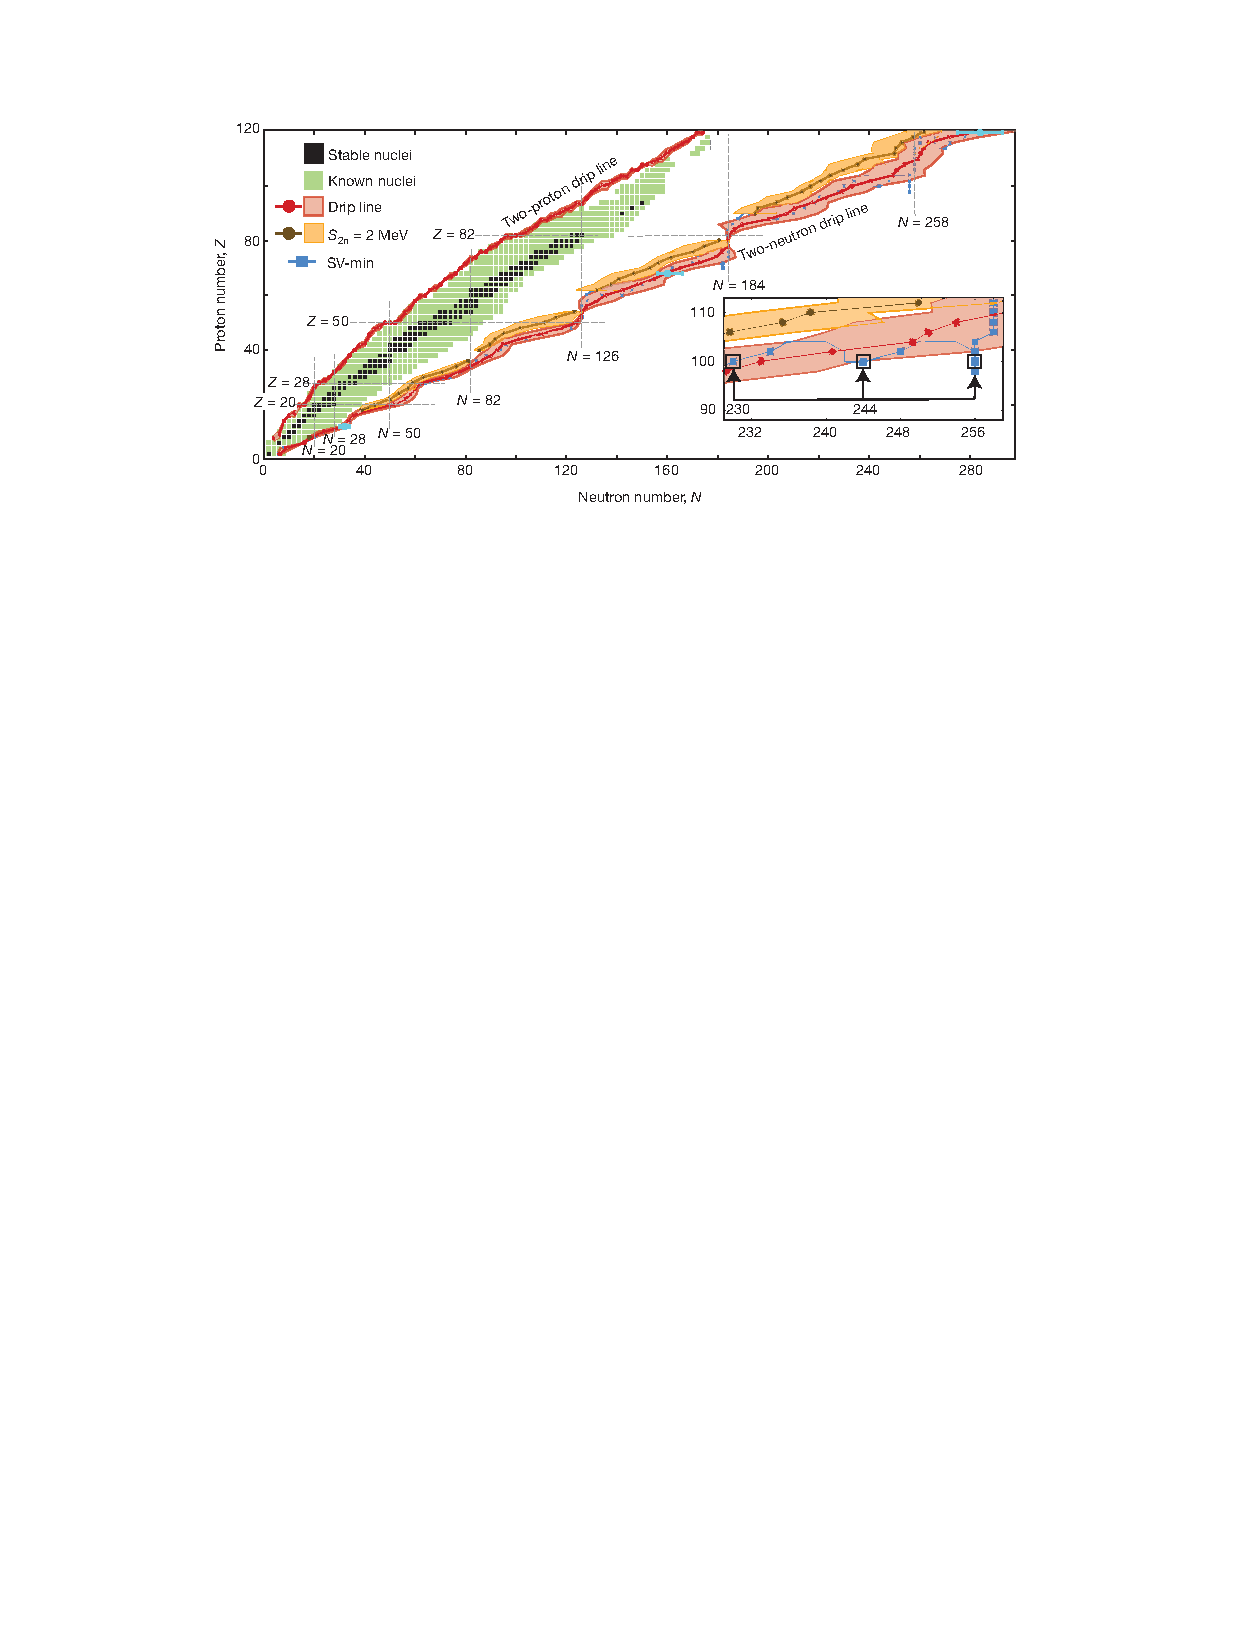
\includegraphics[width=1.0\textwidth]{thesis/doc/images/external/nuclear_landscape_embedded.pdf}
  \caption[
    The nuclear landscape,
    with stable and unstable atomic nuclei denoted by the black and green squares, respectively,
    and a theoretical prediction of the limit of bound nuclei indicated by the red bands.
  ]{
    The nuclear landscape,
    with stable and unstable atomic nuclei denoted by the black and green squares, respectively,
    and a theoretical prediction of the limit of bound nuclei indicated by the red bands.
    Figure taken from Ref.~\cite{Erle12limits}.
  }\label{fig:nuclear_landscape}
\end{figure}

Atomic nuclei consist of protons and neutrons, collectively referred to as nucleons.
The interaction between nucleons is dominated by the strong interaction,
and nuclei as self-bound systems of nucleons form as the result of the strong interaction
overcoming a strong kinetic repulsion
due to nucleons being fermions and obeying the Pauli exclusion principle.
Emergent out of the interplay between these two effects,
with contributions from the weak and electromagnetic interactions,
is the nuclear landscape,
shown in Fig.~\ref{fig:nuclear_landscape}.
All of these isotopes arise out of the same basic physics,
with constituent nucleons interacting via basic two- and three-particle interactions.

\textit{Ab initio} nuclear theory aims to realize this understanding of the nuclear landscape
in theoretical calculations,
determining first the interactions between nucleons
in a way that is connected to the fundamental theory of the strong interaction
and then
modeling nuclei using only the interactions between nucleons as input.
Using only these interactions as inputs means that \abinitio{} methods
have far-reaching predictive power with a large range of applicability.
An additional requirement for the \abinitio{} approach is that
the methods used are in a theoretical limit exact
and thus systematically improvable for any practical approximation.
This feature also allows the \abinitio{} approach to in principle deliver robust uncertainty estimates,
allowing for the meaningful comparison between experiment and theory
and also between different \abinitio{} theoretical approaches.

\begin{figure}[t]
  \centering
  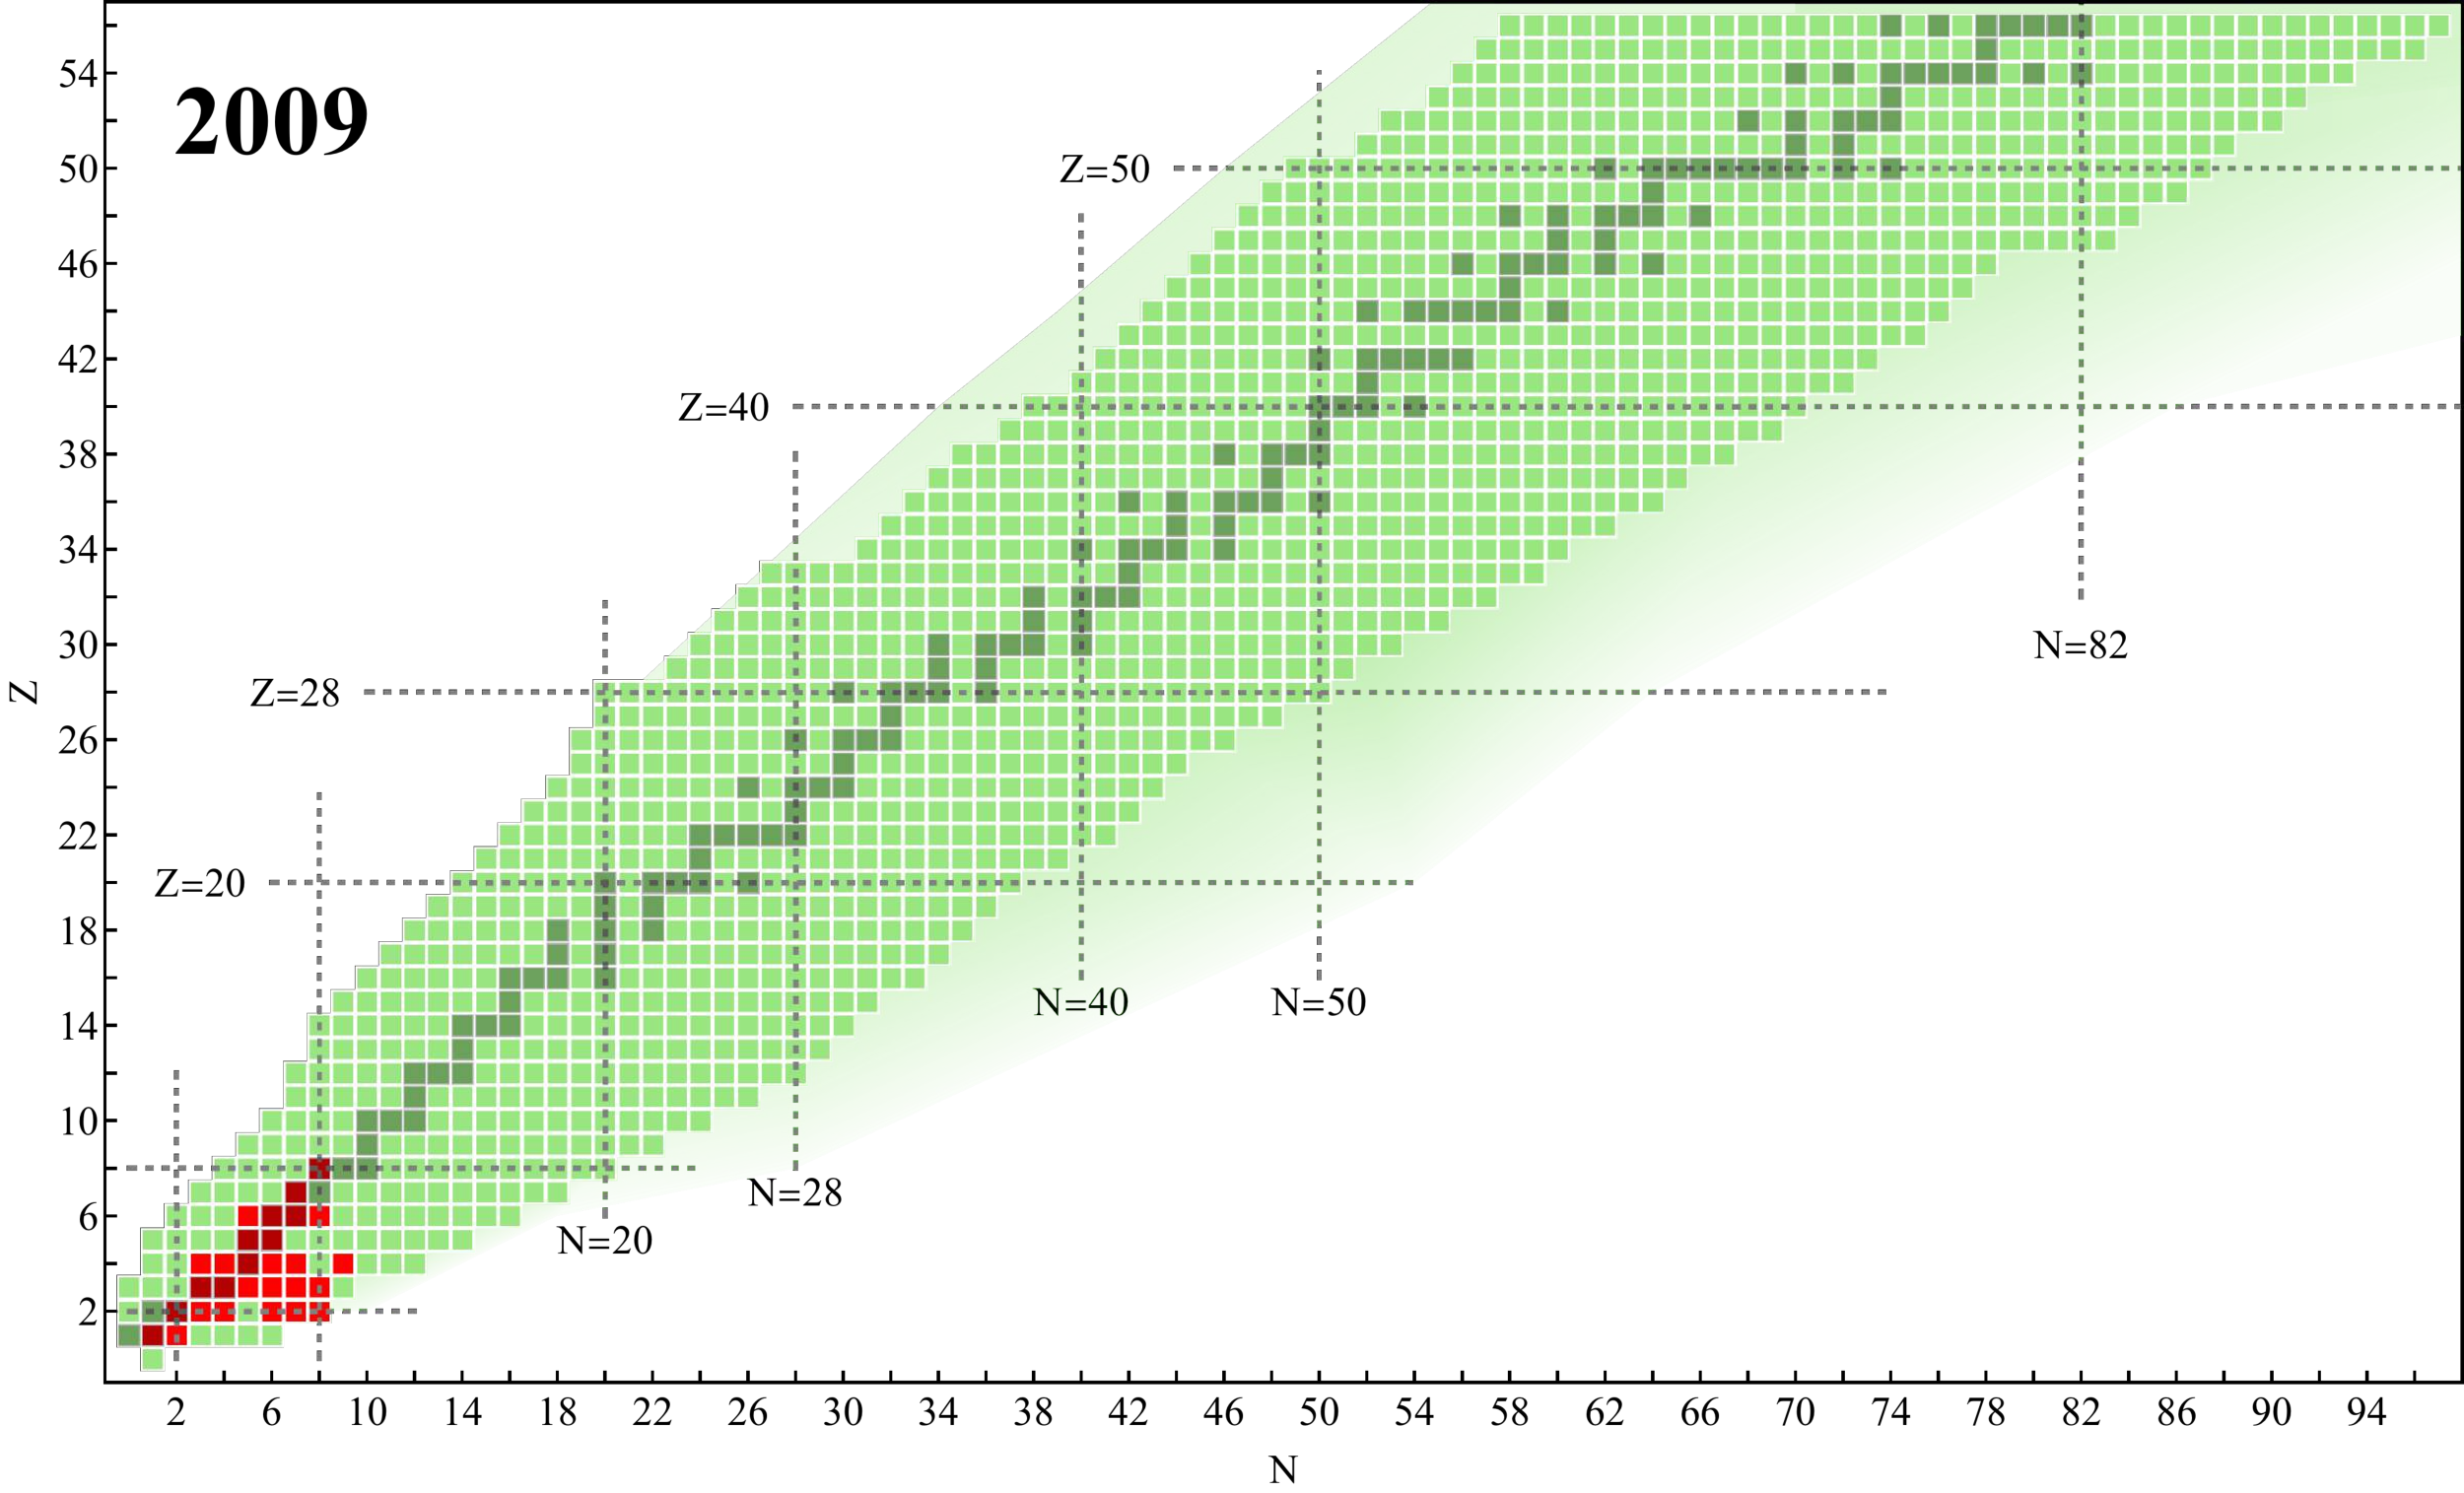
\includegraphics[width=0.45\textwidth]{thesis/doc/images/external/nuclear_chart_2009.pdf}
  \hspace{0cm}
  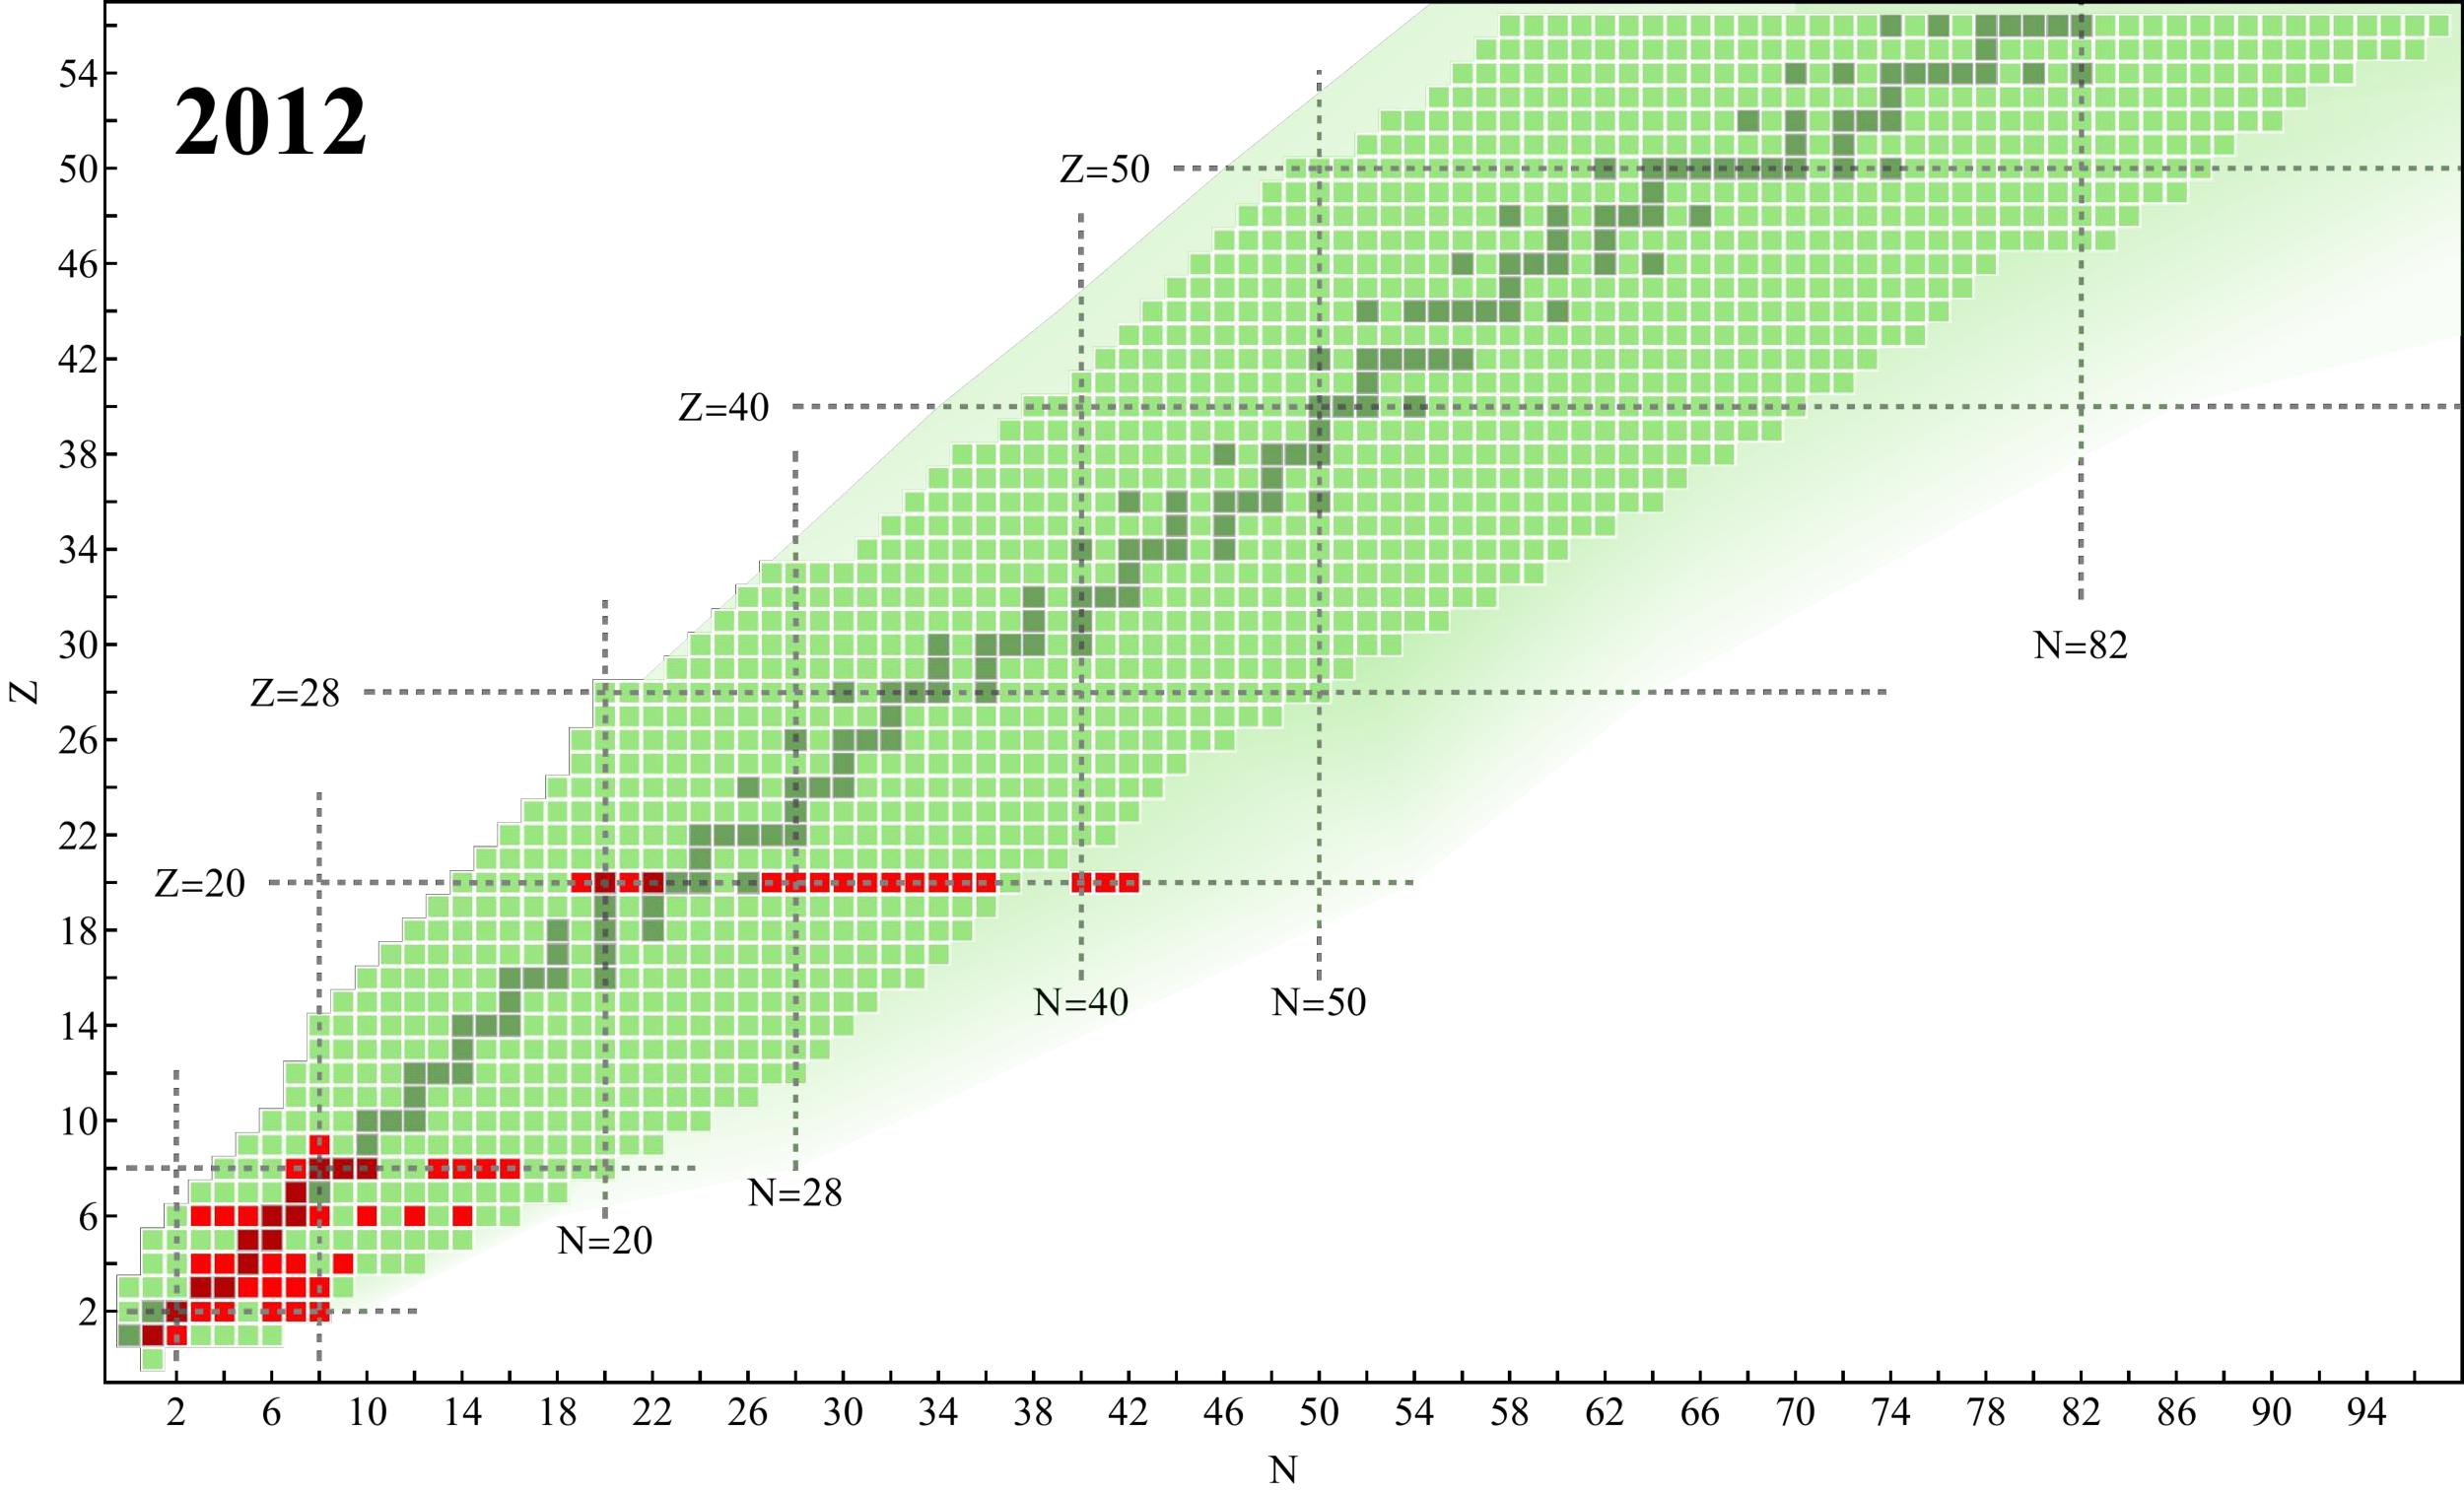
\includegraphics[width=0.45\textwidth]{thesis/doc/images/external/nuclear_chart_2012.pdf}\\
  \vspace{0.05cm}
  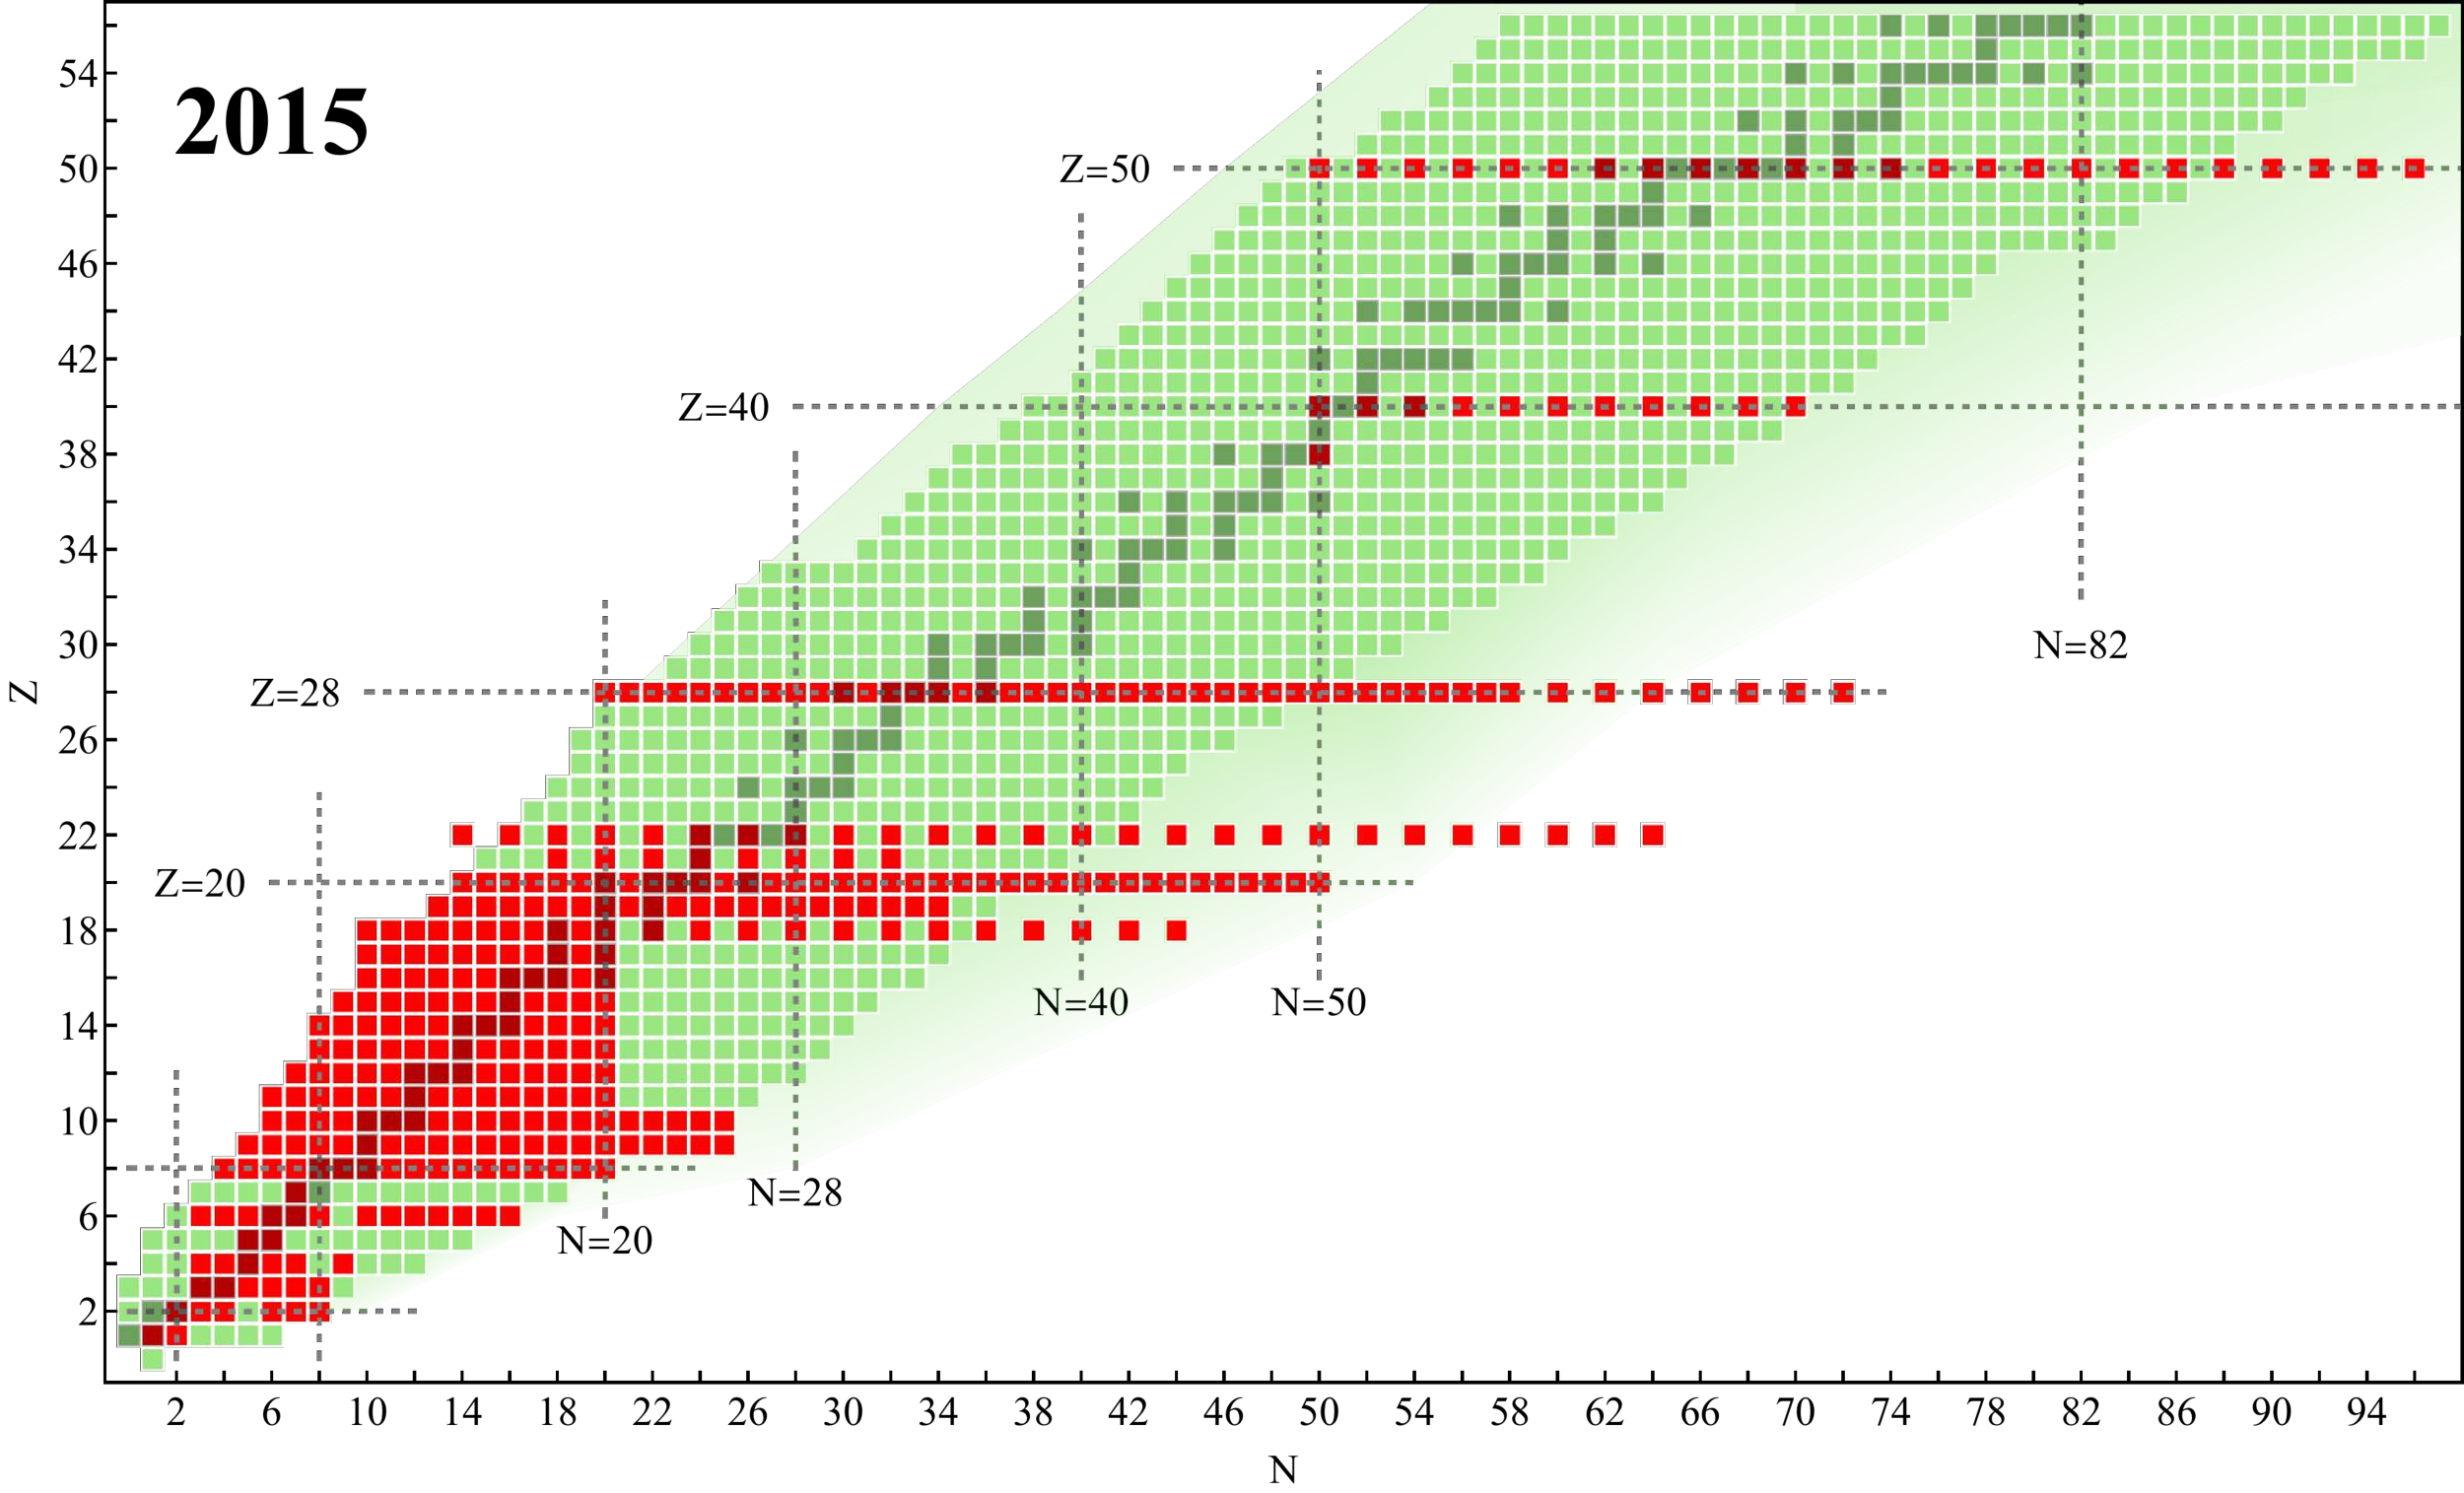
\includegraphics[width=0.45\textwidth]{thesis/doc/images/external/nuclear_chart_2015.pdf}
  \hspace{0cm}
  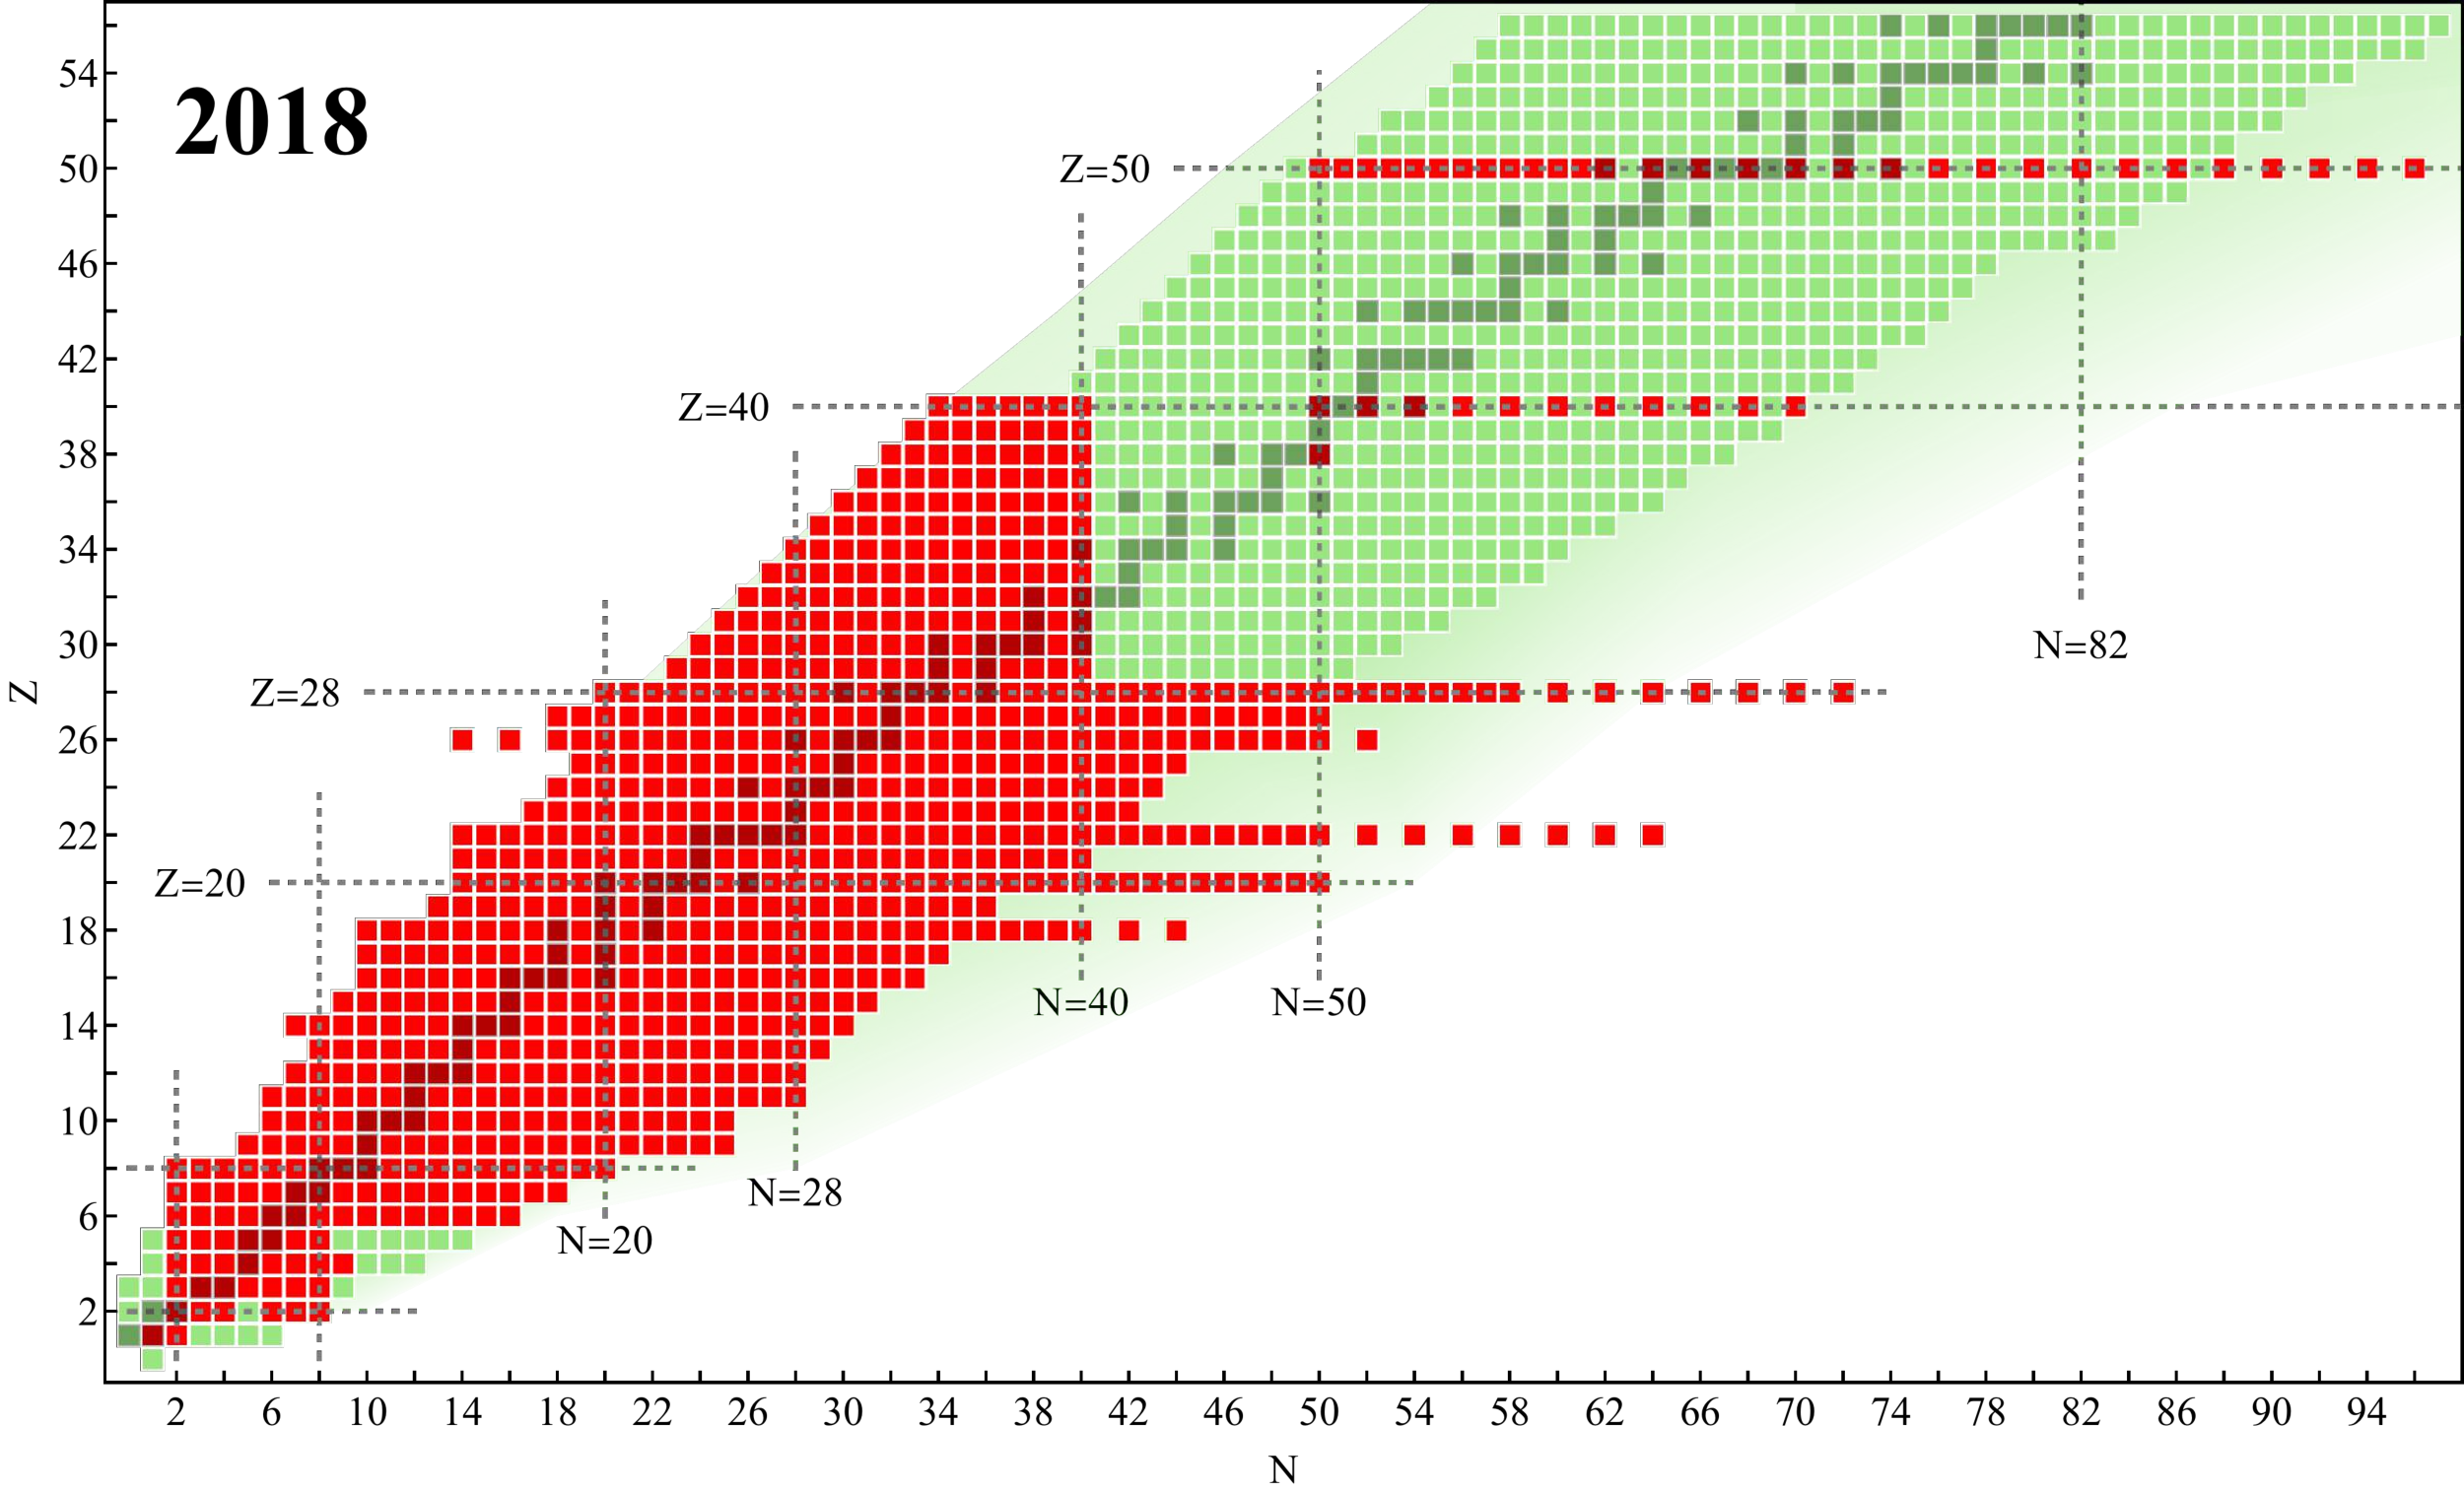
\includegraphics[width=0.45\textwidth]{thesis/doc/images/external/nuclear_chart_2018.pdf}
  \caption[
    Chart of nuclides showing in red nuclei for which \abinitio{} calculations
    involving two- and three-body interactions had been done in 2009 (top left)
    to 2018 (bottom right).
    Only calculations for which convergence with respect to basis size was achieved
    are included in the charts.
  ]{
    Chart of nuclides showing in red nuclei for which \abinitio{} calculations
    involving two- and three-body interactions had been done in 2009 (top left)
    to 2018 (bottom right).
    Only calculations for which convergence with respect to basis size was achieved
    are included in the charts.
    Figure courtesy of Heiko Hergert~\cite{Herg15imsrgphysrep}.
  }\label{fig:ab_initio_conquest}
\end{figure}

Over the past two decades,
the range of \abinitio{} results has expanded rapidly,
as is shown in Fig.~\ref{fig:ab_initio_conquest}.
This change was driven by a shift in our understanding of \textit{low-energy}
nuclear physics,
both in the determination of nuclear interactions
and in the subsequent modeling of nuclei.
The essential change in our understanding of nuclear forces
is encapsulated in the effective field theory (EFT) and renormalization group (RG) methods.
Underlying both of these ideas is the concept of limited resolution in low-energy physics
and the realization that behavior at short distances (small wavelengths or high energies)
does not affect the big picture at long distances.
Effective field theory methods connect to underlying fundamental theories
explicitly setting the scale to include essential long-distance physics
and generating the most general expansion for the short-distance physics
in terms of contact interactions~\cite{Wein78eft,Hamm19nuceftreview,Epel08chiraleft,Mach11chiraleft}.
Renormalization group methods allow for varying of the resolution scale,
decoupling or integrating out high-energy details to produce an efficient low-resolution
description of the system at hand~\cite{Wils71rg,Bogn06srg,Bogn09vlowk}.
These two obviously synergistic methods have worked together to produce
low-resolution nuclear forces rooted in the fundamental theory of quantum chromodynamics.

With these new, more efficient low-energy nuclear forces
and the ever increasing available computational resources,
the parallel development of nuclear many-body methods was uncapped.
New developments on well-established methods,
such as the coupled cluster approach,
and the introduction of new methods,
such as the in-medium similarity renormalization group,
have carried \abinitio{} nuclear theory to its present state.
A crucial role was played by the developments on
many-body expansion methods, such as coupled cluster or
the in-medium similarity renormalization group,
whose computational cost scales polynomially
in the system size
rather than exponentially like
exact diagonalization approaches
or Monte Carlo simulations.
These methods are the best candidates available
for extending the reach of \abinitio{} nuclear theory
to the heavy-mass region
and the neutron-rich medium-mass region.

\section{Goals}

The focus of this work is the in-medium similarity renormalization group (IMSRG)~\cite{Tsuk10imsrg}.
As indicated by its name,
it brings the RG approach of decoupling low- and high-energy states to the many-body problem,
seeking to decouple the state of a system from its elementary excitations.
It is flexible in that it can target both ground states and low-lying excited states
and calculate energies as well as expectation values for other operators,
and while its original formulation centers on describing closed-shell nuclei,
multiple variants are able to model open-shell nuclei
as well~\cite{Stro16vsimsrg,Bogn14vsimsrg,Herg2013mrimsrg,Gebr2016imncsm,Yao18imgcm}.

The current state-of-the-art IMSRG approaches truncate the formalism at the IMSRG(2) level,
the first non-trivial truncation where up to normal-ordered two-body operators are kept in the equations.
This truncation has been quite successful,
but for the purposes of reaching higher precision and allowing for quantification
of many-body uncertainties,
extending the truncation to the IMSRG(3) level is of great interest.
In practice, the general IMSRG(3) is computationally too expensive to allow for
a systematic study in even the smallest systems and model spaces.
By considering only closed-shell systems,
one can apply spherical symmetry to reduce the IMSRG(3)
based on the shared symmetries of the system, the Hamiltonian, and computational basis.
For the IMSRG, this formulation is less restrictive than one may expect,
as the valence-space IMSRG can be used to produce an effective shell-model Hamiltonian
that can be fed into a shell-model code and predict the properties of open-shell nuclei
as well~\cite{Bogn14vsimsrg,Stro16vsimsrg,Holt19vsimsrg_range}.
In this work, we perform the angular-momentum reduction of the IMSRG(3).
We aim to use this to systematically study the improvements offered by the IMSRG(3)
for the ground-state properties of light and medium-mass nuclei.

\section{Outline}

The remainder of this thesis is structured as follows:
\begin{itemize}
  \item{In Chapter~\ref{ch:nuclear_forces},
        we introduce some aspects of the theory of nuclear forces.
        We focus on the modern approaches to deriving nuclear forces
        and
        the construction and generation of low-resolution Hamiltonians
        that improve the convergence of many-body calculations.}
  \item{In Chapter~\ref{ch:many_body},
        we introduce the many-body formalism that underlies the IMSRG.\@
        We introduce some related many-body methods that also build on this formalism
        to help position the IMSRG in the greater space of available many-body methods.}
  \item{In Chapter~\ref{ch:imsrg},
        we discuss the IMSRG in detail.
        We discuss the general formalism and the IMSRG(2) and IMSRG(3) truncations.
        We also discuss generator choice,
        which sets how the IMSRG decouples low and high energies,
        and the Magnus expansion,
        an extension that makes the IMSRG easier to solve and easier to apply to other observables.
        We show some benchmark results for our implementation of the IMSRG(2) for ${}^4\text{He}$.}
  \item{In Chapter~\ref{ch:ang_mom_coupling},
        we introduce the angular-momentum reduction formalism.
        We apply this formalism to the IMSRG(3)
        and some auxiliary many-body operations.
        The result is the IMSRG(3) in a spherically symmetric basis,
        which is computationally more efficient
        and allows us to solve the flow equations
        for light and medium-mass nuclei in small model spaces.}
  \item{In Chapter~\ref{ch:jscheme_results},
        we discuss the contributions of the IMSRG(3) truncation
        to ground-state properties of nuclei
        using the optimized spherically-reduced IMSRG(3).
        We consider how the IMSRG(3) handles different reference state choices,
        and we investigate what the effects of individual contributions to the IMSRG(3) are.}
  \item{In Chapter~\ref{ch:summary},
        we summarize our results
        and offer an outlook for the next steps
        in exploring three-body effects in the IMSRG.}
\end{itemize}
